% Agentic Coding Tools - Part 1: Introduction & Installation
% Complete Beamer Presentation with UofSC Color Scheme
% Author: J. Vaught
% Date: January 2026

\documentclass[aspectratio=169,11pt]{beamer}

% ============================================================================
% THEME AND COLOR CONFIGURATION
% ============================================================================
\usetheme{Madrid}
\usecolortheme{default}

% Remove rounded corners - sharp edges only
\setbeamertemplate{blocks}[default]
\setbeamertemplate{title page}[default][colsep=-4bp,rounded=false,shadow=false]
\setbeamertemplate{frametitle}[default][colsep=-4bp,rounded=false,shadow=false]
\setbeamertemplate{navigation symbols}{}

% UofSC Color Palette
\definecolor{Garnet}{HTML}{73000A}
\definecolor{DarkGarnet}{HTML}{570008}
\definecolor{Rose}{HTML}{CC2E40}
\definecolor{Atlantic}{HTML}{466A9F}
\definecolor{Congaree}{HTML}{1F414D}
\definecolor{Horseshoe}{HTML}{65780B}
\definecolor{Grass}{HTML}{CED318}
\definecolor{Honeycomb}{HTML}{A49137}
\definecolor{Black90}{HTML}{363636}
\definecolor{Black70}{HTML}{5C5C5C}
\definecolor{Black50}{HTML}{A2A2A2}
\definecolor{WarmGrey}{HTML}{676156}
\definecolor{Sandstorm}{HTML}{FFF2E3}
\definecolor{Azalea}{HTML}{844247}

% Apply UofSC colors to Beamer elements
\setbeamercolor{palette primary}{bg=Garnet,fg=white}
\setbeamercolor{palette secondary}{bg=Congaree,fg=white}
\setbeamercolor{palette tertiary}{bg=Atlantic,fg=white}
\setbeamercolor{palette quaternary}{bg=black,fg=white}

\setbeamercolor{structure}{fg=Garnet}
\setbeamercolor{title}{fg=white,bg=Garnet}
\setbeamercolor{frametitle}{fg=white,bg=Garnet}
\setbeamercolor{framesubtitle}{fg=Black70}

\setbeamercolor{block title}{bg=Garnet,fg=white}
\setbeamercolor{block body}{bg=Sandstorm,fg=black}
\setbeamercolor{block title alerted}{bg=Rose,fg=white}
\setbeamercolor{block body alerted}{bg=Sandstorm,fg=black}
\setbeamercolor{block title example}{bg=Congaree,fg=white}
\setbeamercolor{block body example}{bg=Sandstorm,fg=black}

\setbeamercolor{item}{fg=Garnet}
\setbeamercolor{subitem}{fg=Atlantic}
\setbeamercolor{subsubitem}{fg=Congaree}

\setbeamercolor{section in toc}{fg=Garnet}
\setbeamercolor{subsection in toc}{fg=Atlantic}

\setbeamercolor{footline}{bg=Black90,fg=white}
\setbeamercolor{author in head/foot}{bg=Garnet,fg=white}
\setbeamercolor{title in head/foot}{bg=Congaree,fg=white}
\setbeamercolor{date in head/foot}{bg=Atlantic,fg=white}

% ============================================================================
% PACKAGES
% ============================================================================
\usepackage[utf8]{inputenc}
\usepackage[T1]{fontenc}
\usepackage{lmodern}
\usepackage{amsmath,amssymb}
\usepackage{graphicx}
\usepackage{tikz}
\usetikzlibrary{shapes.geometric,arrows.meta,positioning,fit,backgrounds,calc}
\usepackage{listings}
\usepackage{booktabs}
\usepackage{array}
\usepackage{hyperref}
\usepackage{xcolor}
\usepackage{fontawesome5}

% ============================================================================
% LISTINGS CONFIGURATION
% ============================================================================
\lstset{
    basicstyle=\ttfamily\scriptsize,
    backgroundcolor=\color{Sandstorm},
    keywordstyle=\color{Garnet}\bfseries,
    commentstyle=\color{Black50}\itshape,
    stringstyle=\color{Congaree},
    numberstyle=\tiny\color{Black70},
    numbers=left,
    numbersep=5pt,
    breaklines=true,
    frame=single,
    frameround=ffff,
    rulecolor=\color{Black70},
    showstringspaces=false,
    tabsize=2,
    captionpos=b,
    xleftmargin=0.5cm,
    xrightmargin=0.5cm
}

\lstdefinestyle{bash}{
    language=bash,
    morekeywords={brew,pip,npm,export,echo,source,git,cd,mkdir,wget,sudo,dpkg,chmod,python,python3,aider,claude,openai,ollama,curl}
}

\lstdefinestyle{python}{
    language=Python,
    morekeywords={import,from,as,def,class,return,if,else,for,in,with,open,print}
}

% ============================================================================
% TIKZ STYLES
% ============================================================================
\tikzset{
    % Sharp corners, no rounded edges
    agentbox/.style={
        rectangle,
        draw=Garnet,
        fill=white,
        thick,
        minimum width=4cm,
        minimum height=1cm,
        align=center,
        font=\small
    },
    agentboxfill/.style={
        rectangle,
        draw=Garnet,
        fill=Sandstorm,
        thick,
        minimum width=4cm,
        minimum height=1cm,
        align=center,
        font=\small
    },
    toolbox/.style={
        rectangle,
        draw=Atlantic,
        fill=white,
        thick,
        minimum width=2.5cm,
        minimum height=0.8cm,
        align=center,
        font=\scriptsize
    },
    categorybox/.style={
        rectangle,
        draw=Congaree,
        fill=Sandstorm,
        thick,
        minimum width=3.5cm,
        minimum height=0.7cm,
        align=center,
        font=\small
    },
    arrow/.style={
        ->,
        >=stealth,
        thick,
        color=Garnet
    },
    dashedarrow/.style={
        ->,
        >=stealth,
        dashed,
        thick,
        color=Atlantic
    }
}

% ============================================================================
% TITLE PAGE INFORMATION
% ============================================================================
\title[Agentic Coding Tools]{Agentic Coding Tools}
\subtitle{Part 1: Introduction \& Installation}
\author{J. Vaught}
\institute{University of South Carolina}
\date{January 2026}

% ============================================================================
% DOCUMENT BEGIN
% ============================================================================
\begin{document}

% ----------------------------------------------------------------------------
% TITLE SLIDE
% ----------------------------------------------------------------------------
\begin{frame}[plain]
    \titlepage
    \begin{center}
        \small A comprehensive guide to autonomous coding assistants\\
        Covering 15+ tools and frameworks
    \end{center}
\end{frame}

% ----------------------------------------------------------------------------
% TABLE OF CONTENTS
% ----------------------------------------------------------------------------
\begin{frame}{Outline}
    \tableofcontents
\end{frame}

% ============================================================================
% SECTION 1: WHAT ARE AGENTIC CODING TOOLS?
% ============================================================================
\section{What are Agentic Coding Tools?}

% ----------------------------------------------------------------------------
\begin{frame}{Understanding Agentic Coding Tools}
    \begin{columns}[T]
        \begin{column}{0.55\textwidth}
            \textbf{Definition:}
            \begin{itemize}
                \item Autonomous software agents using AI for code development
                \item Go beyond simple code completion---they \textbf{take actions}
                \item Read files, execute commands, run tests, install dependencies
                \item Multi-turn conversations with context awareness
            \end{itemize}
        \end{column}
        \begin{column}{0.45\textwidth}
            \begin{block}{Key Characteristics}
                \begin{enumerate}
                    \item \textcolor{Garnet}{\textbf{Autonomous Action}}
                    \item \textcolor{Garnet}{\textbf{Context Awareness}}
                    \item \textcolor{Garnet}{\textbf{Tool Integration}}
                    \item \textcolor{Garnet}{\textbf{Iterative Problem Solving}}
                    \item \textcolor{Garnet}{\textbf{Multi-step Reasoning}}
                \end{enumerate}
            \end{block}
        \end{column}
    \end{columns}

    \vspace{0.3cm}
    \begin{alertblock}{Paradigm Shift}
        Instead of copy-pasting suggestions, you \textbf{describe what you want} and the agent figures out how to accomplish it.
    \end{alertblock}

    \note{The fundamental difference between agentic tools and traditional code completion is agency. Traditional tools suggest code snippets. Agentic tools execute commands, read your codebase, run tests, debug issues, commit changes, and manage dependencies.}
\end{frame}

% ----------------------------------------------------------------------------
\begin{frame}{How Agentic Tools Work: The Agent Loop}
    \begin{center}
        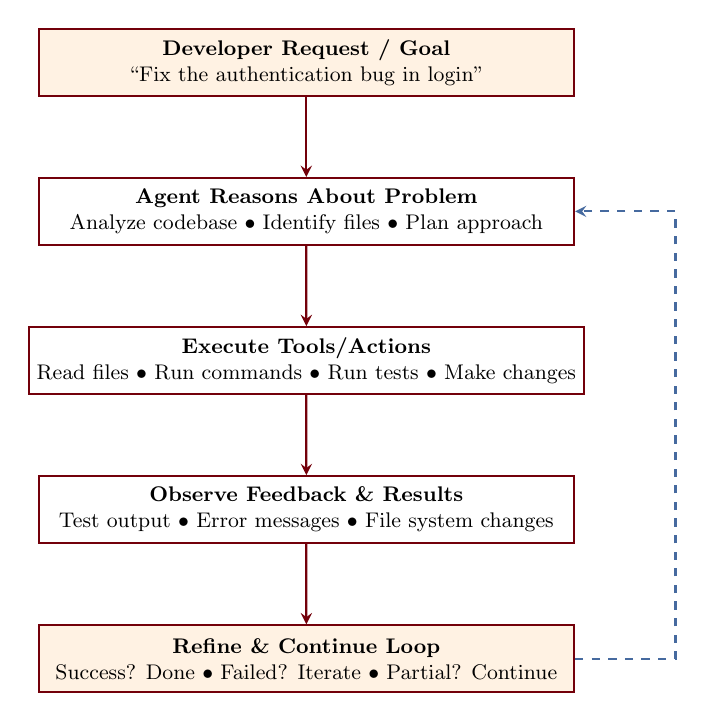
\begin{tikzpicture}[node distance=1.2cm, scale=0.85, transform shape]
            % Developer Request
            \node[agentboxfill, minimum width=8cm] (request) {
                \textbf{Developer Request / Goal}\\
                \small ``Fix the authentication bug in login''
            };

            % Reasoning
            \node[agentbox, below=of request, minimum width=8cm] (reason) {
                \textbf{Agent Reasons About Problem}\\
                \small Analyze codebase $\bullet$ Identify files $\bullet$ Plan approach
            };

            % Execute
            \node[agentbox, below=of reason, minimum width=8cm] (execute) {
                \textbf{Execute Tools/Actions}\\
                \small Read files $\bullet$ Run commands $\bullet$ Run tests $\bullet$ Make changes
            };

            % Observe
            \node[agentbox, below=of execute, minimum width=8cm] (observe) {
                \textbf{Observe Feedback \& Results}\\
                \small Test output $\bullet$ Error messages $\bullet$ File system changes
            };

            % Refine
            \node[agentboxfill, below=of observe, minimum width=8cm] (refine) {
                \textbf{Refine \& Continue Loop}\\
                \small Success? Done $\bullet$ Failed? Iterate $\bullet$ Partial? Continue
            };

            % Arrows (straight lines only)
            \draw[arrow] (request) -- (reason);
            \draw[arrow] (reason) -- (execute);
            \draw[arrow] (execute) -- (observe);
            \draw[arrow] (observe) -- (refine);

            % Loop back arrow (right angle)
            \draw[dashedarrow] (refine.east) -- ++(1.5,0) |- (reason.east);
        \end{tikzpicture}
    \end{center}

    \note{The agentic loop is the core concept. Unlike traditional IDEs where you're in control, with agentic tools you describe the goal and the agent reasons through how to achieve it.}
\end{frame}

% ----------------------------------------------------------------------------
\begin{frame}{Example: Fixing a Bug with an Agent}
    \textbf{Scenario:} ``Fix the login endpoint---it's returning 500 errors''

    \vspace{0.3cm}
    \begin{columns}[T]
        \begin{column}{0.5\textwidth}
            \begin{block}{1. Exploration Phase (2--3 min)}
                \begin{itemize}
                    \item Search codebase for login files
                    \item Examine error logs
                    \item Identify dependencies
                    \item Read authentication logic
                \end{itemize}
            \end{block}

            \begin{block}{2. Analysis Phase (1--2 min)}
                \begin{itemize}
                    \item Understand the problem
                    \item Check recent commits
                    \item Review test files
                \end{itemize}
            \end{block}
        \end{column}
        \begin{column}{0.5\textwidth}
            \begin{block}{3. Implementation Phase (3--5 min)}
                \begin{itemize}
                    \item Propose fixes
                    \item Write code changes
                    \item Run tests automatically
                \end{itemize}
            \end{block}

            \begin{block}{4. Verification Phase (2--3 min)}
                \begin{itemize}
                    \item Execute full test suite
                    \item Check for regressions
                    \item Commit changes with git
                \end{itemize}
            \end{block}
        \end{column}
    \end{columns}

    \vspace{0.2cm}
    \begin{exampleblock}{Result}
        Bug fixed, tests passing, changes committed---all without manual intervention
    \end{exampleblock}

    \note{This separates agentic tools from static code completion. A traditional AI might suggest a one-line fix. An agentic tool navigates your codebase, writes comprehensive fixes, runs tests, and verifies everything works.}
\end{frame}

% ----------------------------------------------------------------------------
\begin{frame}{Benefits of Agentic Coding Tools}
    \begin{columns}[T]
        \begin{column}{0.5\textwidth}
            \begin{block}{Productivity Benefits}
                \begin{itemize}
                    \item 40--60\% faster for certain tasks
                    \item Eliminates context switching
                    \item Automated testing/verification
                    \item Faster debugging
                \end{itemize}
            \end{block}

            \begin{block}{Quality Benefits}
                \begin{itemize}
                    \item Comprehensive code review
                    \item Automated test generation
                    \item Consistent code style
                    \item Better documentation
                \end{itemize}
            \end{block}
        \end{column}
        \begin{column}{0.5\textwidth}
            \begin{block}{Learning Benefits}
                \begin{itemize}
                    \item Step-by-step problem solving
                    \item Best practices demonstrated
                    \item Interactive feedback
                    \item Explore alternatives
                \end{itemize}
            \end{block}

            \begin{alertblock}{Limitations}
                \begin{itemize}
                    \item Context window limits
                    \item Hallucination risk
                    \item API costs add up
                    \item Learning curve varies
                \end{itemize}
            \end{alertblock}
        \end{column}
    \end{columns}

    \note{These tools are force multipliers, not magic wands. They excel at routine tasks but struggle with deep architectural decisions and security-critical code.}
\end{frame}

% ----------------------------------------------------------------------------
\begin{frame}{Traditional vs. Agentic Tools}
    \begin{center}
        \small
        \begin{tabular}{@{}l p{4.5cm} p{5cm}@{}}
            \toprule
            \textbf{Aspect} & \textbf{Traditional (Copilot)} & \textbf{Agentic (Claude Code, Aider)} \\
            \midrule
            \textbf{Input} & Type code, get suggestions & Describe task in natural language \\
            \textbf{Output} & Code snippets & Complete solutions with verification \\
            \textbf{Scope} & Single file, current context & Entire codebase \\
            \textbf{Actions} & Suggest code & Execute commands, modify files, run tests \\
            \textbf{Verification} & Manual testing & Automatic testing and validation \\
            \textbf{Error Recovery} & You fix errors & Agent attempts fixes automatically \\
            \textbf{Use Case} & Writing new code & Solving problems, refactoring, debugging \\
            \bottomrule
        \end{tabular}
    \end{center}

    \vspace{0.3cm}
    \begin{exampleblock}{Complementary Tools}
        Agentic tools are \textbf{not replacements}---they're complementary. Use Copilot for autocomplete while coding, then Claude Code for ``refactor this entire module.''
    \end{exampleblock}

    \note{Different tools excel at different tasks. Understanding when to use each is key to productivity.}
\end{frame}

% ============================================================================
% SECTION 2: THE THREE CATEGORIES OVERVIEW
% ============================================================================
\section{The Three Categories Overview}

% ----------------------------------------------------------------------------
\begin{frame}{The Agentic Tools Ecosystem}
    \begin{center}
        \begin{tikzpicture}[node distance=0.8cm, scale=0.75, transform shape]
            % Root
            \node[agentboxfill, minimum width=6cm, minimum height=1cm] (root) {
                \textbf{AGENTIC TOOLS ECOSYSTEM}
            };

            % Three categories
            \node[categorybox, below left=1.2cm and 0.5cm of root, minimum width=4cm] (terminal) {
                \faTerminal\ \textbf{Terminal-Based Agents}
            };
            \node[categorybox, below=1.2cm of root, minimum width=4cm] (ide) {
                \faCode\ \textbf{Agentic IDEs}
            };
            \node[categorybox, below right=1.2cm and 0.5cm of root, minimum width=4cm] (vscode) {
                \faPuzzlePiece\ \textbf{VS Code Plugins}
            };

            % Terminal tools
            \node[toolbox, below=0.6cm of terminal, xshift=-1cm] (claude) {Claude Code};
            \node[toolbox, right=0.2cm of claude] (aider) {Aider};
            \node[toolbox, below=0.3cm of claude] (codex) {Codex CLI};
            \node[toolbox, right=0.2cm of codex] (gemini) {Gemini CLI};

            % IDE tools
            \node[toolbox, below=0.6cm of ide, xshift=-0.8cm] (cursor) {Cursor};
            \node[toolbox, right=0.2cm of cursor] (windsurf) {Windsurf};
            \node[toolbox, below=0.3cm of cursor, xshift=0.4cm] (zed) {Zed};

            % VS Code tools
            \node[toolbox, below=0.6cm of vscode, xshift=-1cm] (copilot) {GitHub Copilot};
            \node[toolbox, right=0.2cm of copilot] (cline) {Cline};
            \node[toolbox, below=0.3cm of copilot] (continue) {Continue};
            \node[toolbox, right=0.2cm of continue] (amazonq) {Amazon Q};

            % Arrows from root
            \draw[arrow] (root.south) -- ++(0,-0.3) -| (terminal.north);
            \draw[arrow] (root.south) -- (ide.north);
            \draw[arrow] (root.south) -- ++(0,-0.3) -| (vscode.north);

            % Descriptions
            \node[below=2.5cm of terminal, text width=3.5cm, align=center, font=\tiny] {
                Full system access\\Command line interface
            };
            \node[below=2.5cm of ide, text width=3.5cm, align=center, font=\tiny] {
                Purpose-built editors\\Optimized UX
            };
            \node[below=2.5cm of vscode, text width=3.5cm, align=center, font=\tiny] {
                Add to existing editor\\Familiar environment
            };
        \end{tikzpicture}
    \end{center}

    \note{Terminal-based agents are most powerful for complex tasks and automation. Agentic IDEs provide cohesive, optimized experience. VS Code plugins integrate agents into your existing editor.}
\end{frame}

% ----------------------------------------------------------------------------
\begin{frame}{Category 1: Terminal-Based Agents}
    \begin{columns}[T]
        \begin{column}{0.5\textwidth}
            \begin{block}{What Are They?}
                \begin{itemize}
                    \item Run in your terminal/command line
                    \item Full access to system and codebase
                    \item Natural language communication
                    \item Execute any command you could
                    \item Multi-turn conversations
                \end{itemize}
            \end{block}

            \begin{block}{Why Most Powerful?}
                \begin{enumerate}
                    \item \textbf{Unrestricted Access}
                    \item \textbf{Scripting Integration}
                    \item \textbf{Version Control}
                    \item \textbf{Automation}
                    \item \textbf{Flexibility}
                \end{enumerate}
            \end{block}
        \end{column}
        \begin{column}{0.5\textwidth}
            \begin{exampleblock}{Best For}
                \begin{itemize}
                    \item Complex multi-step tasks
                    \item Automation and scripting
                    \item Git integration
                    \item Headless environments
                    \item Development workflows
                \end{itemize}
            \end{exampleblock}

            \begin{alertblock}{Trade-offs}
                \begin{itemize}
                    \item No visual IDE features
                    \item Require terminal comfort
                    \item Context shown in text only
                    \item May need explicit instructions
                \end{itemize}
            \end{alertblock}
        \end{column}
    \end{columns}

    \note{Terminal-based agents are like having a senior developer on your team who works at the command line. Once you master terminal agents, the IDE-based tools feel like simplified versions.}
\end{frame}

% ----------------------------------------------------------------------------
\begin{frame}{Claude Code: Anthropic's Terminal Agent}
    \begin{columns}[T]
        \begin{column}{0.5\textwidth}
            \begin{block}{Overview}
                \begin{itemize}
                    \item Developed by Anthropic
                    \item Uses Claude language models
                    \item Most sophisticated agentic capabilities
                    \item MCP (Model Context Protocol) support
                \end{itemize}
            \end{block}

            \begin{block}{Key Strengths}
                \begin{itemize}
                    \item Best long-context understanding
                    \item Excellent code analysis
                    \item Strong reasoning for complex problems
                    \item Multi-hour conversations
                    \item Web search and tool use
                \end{itemize}
            \end{block}
        \end{column}
        \begin{column}{0.5\textwidth}
            \begin{exampleblock}{Best Use Cases}
                \begin{itemize}
                    \item Large refactoring projects
                    \item Complex debugging
                    \item Architectural discussions
                    \item Building from specifications
                    \item Learning and exploration
                \end{itemize}
            \end{exampleblock}

            \begin{block}{Resource Requirements}
                \begin{itemize}
                    \item Terminal + API access
                    \item Requires API key (paid)
                    \item No heavyweight IDE needed
                \end{itemize}
            \end{block}
        \end{column}
    \end{columns}

    \note{Claude Code's primary advantage is the quality of Claude's reasoning---exceptional at understanding nuanced problems and maintaining context over long conversations.}
\end{frame}

% ----------------------------------------------------------------------------
\begin{frame}{Aider: Open Source Powerhouse}
    \begin{columns}[T]
        \begin{column}{0.5\textwidth}
            \begin{block}{Overview}
                \begin{itemize}
                    \item Open-source (GPLv3)
                    \item Mature, well-maintained
                    \item Multiple LLM providers
                    \item Designed for pair programming
                \end{itemize}
            \end{block}

            \begin{block}{Supported Providers}
                \begin{itemize}
                    \item OpenAI (GPT-4, GPT-3.5)
                    \item Anthropic Claude models
                    \item \textbf{Local models via Ollama}
                    \item Google Gemini
                    \item Mistral, Cohere, others
                \end{itemize}
            \end{block}
        \end{column}
        \begin{column}{0.5\textwidth}
            \begin{exampleblock}{Key Strengths}
                \begin{itemize}
                    \item Works \textbf{offline} with local models
                    \item Multi-file editing with clear diffs
                    \item Excellent git integration
                    \item Active community
                    \item Cost-effective options
                \end{itemize}
            \end{exampleblock}

            \begin{block}{Unique Features}
                \begin{itemize}
                    \item ``Whole file'' mode for rewrites
                    \item Diff-based editing
                    \item Built-in code review
                    \item Completely offline operation
                \end{itemize}
            \end{block}
        \end{column}
    \end{columns}

    \note{Aider is fantastic for open-source advocates or those wanting local models. The diff-based approach is excellent for code review---you always know exactly what the agent changed.}
\end{frame}

% ----------------------------------------------------------------------------
\begin{frame}{Codex CLI \& Gemini CLI}
    \begin{columns}[T]
        \begin{column}{0.5\textwidth}
            \begin{block}{Codex CLI (OpenAI)}
                \textbf{Overview:}
                \begin{itemize}
                    \item OpenAI's official terminal tool
                    \item Access to GPT-4 models
                    \item Optimized for speed
                \end{itemize}

                \textbf{Best For:}
                \begin{itemize}
                    \item Quick code generation
                    \item Command-line tool building
                    \item Script automation
                    \item Fast feedback loops
                \end{itemize}

                \textbf{Limitations:}
                \begin{itemize}
                    \item Less agentic than alternatives
                    \item Fixed context window
                    \item Primarily code generation
                \end{itemize}
            \end{block}
        \end{column}
        \begin{column}{0.5\textwidth}
            \begin{block}{Gemini CLI (Google)}
                \textbf{Overview:}
                \begin{itemize}
                    \item Google's terminal interface
                    \item Gemini 1.5 Pro/Flash models
                    \item \textcolor{Garnet}{\textbf{1 million token context}}
                \end{itemize}

                \textbf{Best For:}
                \begin{itemize}
                    \item Large codebase analysis
                    \item Multi-hour debugging
                    \item Cost-conscious orgs
                    \item Document-heavy workflows
                \end{itemize}

                \textbf{Unique:}
                \begin{itemize}
                    \item 1M token context window
                    \item Good multimodal support
                    \item Competitive pricing
                \end{itemize}
            \end{block}
        \end{column}
    \end{columns}

    \note{Codex CLI is good for speed on well-defined problems. Gemini CLI's 1M token context is game-changing for large-scale refactoring or understanding massive projects.}
\end{frame}

% ----------------------------------------------------------------------------
\begin{frame}{Other Terminal Agents (Brief Overview)}
    \begin{columns}[T]
        \begin{column}{0.5\textwidth}
            \begin{block}{GitHub Copilot CLI}
                \begin{itemize}
                    \item GitHub ecosystem integration
                    \item Good for GitHub workflows
                    \item Fewer agentic features
                \end{itemize}
            \end{block}

            \begin{block}{OpenHands}
                \begin{itemize}
                    \item Open-source agent framework
                    \item Supports multiple backends
                    \item Good for research
                \end{itemize}
            \end{block}
        \end{column}
        \begin{column}{0.5\textwidth}
            \begin{block}{Goose}
                \begin{itemize}
                    \item Lightweight open-source agent
                    \item Python-based, hackable
                    \item Good for learning
                \end{itemize}
            \end{block}

            \begin{block}{Continue CLI}
                \begin{itemize}
                    \item Part of Continue.dev
                    \item VS Code-focused but has CLI
                    \item Emerging as contender
                \end{itemize}
            \end{block}
        \end{column}
    \end{columns}

    \vspace{0.2cm}
    \begin{exampleblock}{Recommendation}
        Focus on Claude Code, Aider, Codex CLI, and Gemini CLI. Monitor these four for future developments.
    \end{exampleblock}

    \note{These tools are worth monitoring but not the primary focus. The main four represent the most mature and powerful options.}
\end{frame}

% ----------------------------------------------------------------------------
\begin{frame}{Category 2: Agentic IDEs}
    \begin{columns}[T]
        \begin{column}{0.55\textwidth}
            \begin{block}{What Are Agentic IDEs?}
                \begin{itemize}
                    \item Purpose-built editors with agents built-in
                    \item No plugins or extensions needed
                    \item Optimized UI for agentic workflows
                    \item Visual code editing + agent capabilities
                \end{itemize}
            \end{block}

            \begin{block}{The Three Main Players}
                \textbf{Cursor} --- Best entry point
                \begin{itemize}
                    \item Based on VS Code, easiest learning curve
                \end{itemize}

                \textbf{Windsurf} --- Most advanced
                \begin{itemize}
                    \item Most sophisticated agent capabilities
                \end{itemize}

                \textbf{Zed} --- Highest performance
                \begin{itemize}
                    \item Rust-based, very fast
                \end{itemize}
            \end{block}
        \end{column}
        \begin{column}{0.45\textwidth}
            \small
            \begin{center}
                \begin{tabular}{@{}l c c@{}}
                    \toprule
                    \textbf{Feature} & \textbf{Terminal} & \textbf{IDE} \\
                    \midrule
                    IDE features & No & Yes \\
                    Visual UI & No & Yes \\
                    Scripting & Excellent & Limited \\
                    Learning & Medium & Low \\
                    Flexibility & Very high & Medium \\
                    \bottomrule
                \end{tabular}
            \end{center}

            \vspace{0.3cm}
            \begin{alertblock}{Trade-off}
                IDEs are great for pure development workflows but less suited to automation and scripting.
            \end{alertblock}
        \end{column}
    \end{columns}

    \note{Agentic IDEs are fantastic for pure development workflows. Many developers use both---terminal agents for heavy lifting, IDE plugins for everyday development.}
\end{frame}

% ----------------------------------------------------------------------------
\begin{frame}{Category 3: VS Code Plugins}
    \begin{columns}[T]
        \begin{column}{0.5\textwidth}
            \begin{block}{Why VS Code Plugins?}
                \begin{itemize}
                    \item Keep your existing editor
                    \item Lower barrier to entry
                    \item Many free/freemium options
                    \item Easy to compare tools
                    \item Familiar environment
                \end{itemize}
            \end{block}

            \begin{exampleblock}{GitHub Copilot}
                \begin{itemize}
                    \item Most widely used
                    \item Excellent completion + chat
                    \item GitHub integration
                    \item \$10/month
                \end{itemize}
            \end{exampleblock}

            \begin{block}{Cline}
                \begin{itemize}
                    \item Strong agentic capabilities
                    \item Multi-file changes
                    \item Free/freemium
                \end{itemize}
            \end{block}
        \end{column}
        \begin{column}{0.5\textwidth}
            \begin{block}{Continue}
                \begin{itemize}
                    \item Hackable and extensible
                    \item Works with any LLM
                    \item Open-source option
                \end{itemize}
            \end{block}

            \begin{block}{Amazon Q}
                \begin{itemize}
                    \item AWS integration
                    \item Enterprise focus
                    \item Free tier available
                \end{itemize}
            \end{block}

            \vspace{0.2cm}
            \begin{alertblock}{Entry Point}
                VS Code plugins are the most accessible entry point. Many developers start here, then graduate to terminal agents for complex tasks.
            \end{alertblock}
        \end{column}
    \end{columns}

    \note{VS Code plugins are the easiest entry point for new users. Many developers use Copilot for everyday coding, then switch to more agentic tools for complex tasks.}
\end{frame}

% ----------------------------------------------------------------------------
\begin{frame}{Decision Framework: Which Tool to Use?}
    \begin{center}
        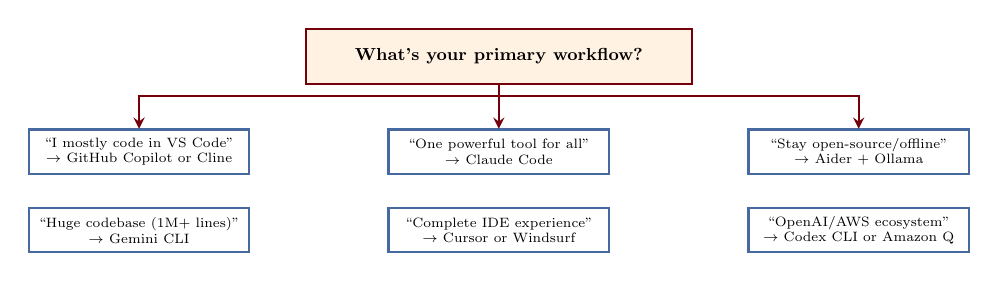
\begin{tikzpicture}[
            node distance=0.6cm,
            scale=0.7,
            transform shape,
            decision/.style={agentboxfill, minimum width=7cm, font=\small},
            answer/.style={toolbox, minimum width=4cm, font=\scriptsize}
        ]
            \node[decision] (q) {\textbf{What's your primary workflow?}};

            \node[answer, below left=0.8cm and 1cm of q] (vscode) {
                ``I mostly code in VS Code''\\
                $\rightarrow$ GitHub Copilot or Cline
            };

            \node[answer, below=0.8cm of q] (powerful) {
                ``One powerful tool for all''\\
                $\rightarrow$ Claude Code
            };

            \node[answer, below right=0.8cm and 1cm of q] (opensource) {
                ``Stay open-source/offline''\\
                $\rightarrow$ Aider + Ollama
            };

            \node[answer, below=0.6cm of vscode] (huge) {
                ``Huge codebase (1M+ lines)''\\
                $\rightarrow$ Gemini CLI
            };

            \node[answer, below=0.6cm of powerful] (ide) {
                ``Complete IDE experience''\\
                $\rightarrow$ Cursor or Windsurf
            };

            \node[answer, below=0.6cm of opensource] (ecosystem) {
                ``OpenAI/AWS ecosystem''\\
                $\rightarrow$ Codex CLI or Amazon Q
            };

            % Arrows
            \draw[arrow] (q.south) -- ++(0,-0.2) -| (vscode.north);
            \draw[arrow] (q.south) -- (powerful.north);
            \draw[arrow] (q.south) -- ++(0,-0.2) -| (opensource.north);
        \end{tikzpicture}
    \end{center}

    \vspace{0.2cm}
    \begin{block}{Recommendation for This Course}
        \begin{enumerate}
            \item Set up \textbf{Claude Code} (primary tool)
            \item Try \textbf{Aider} (open-source alternative)
            \item Experiment with \textbf{Cursor} (IDE experience)
        \end{enumerate}
    \end{block}

    \note{There's no single ``best'' tool---it depends on your priorities. Most professional developers use multiple tools for different situations.}
\end{frame}

% ============================================================================
% SECTION 3: TERMINAL AGENTS INSTALLATION
% ============================================================================
\section{Terminal Agents Installation}

% ----------------------------------------------------------------------------
\begin{frame}{Installation Overview}
    \begin{columns}[T]
        \begin{column}{0.5\textwidth}
            \begin{block}{What We'll Cover}
                \begin{enumerate}
                    \item \textbf{Claude Code} (5--6 slides)
                    \item \textbf{Aider} (3--4 slides)
                    \item \textbf{Codex CLI} (2--3 slides)
                    \item \textbf{Gemini CLI} (3--4 slides)
                    \item \textbf{Others} (1--2 slides)
                \end{enumerate}
            \end{block}

            \begin{alertblock}{Estimated Time}
                30--45 minutes for full setup
            \end{alertblock}
        \end{column}
        \begin{column}{0.5\textwidth}
            \begin{center}
                \begin{tikzpicture}[
                    node distance=0.5cm,
                    scale=0.8,
                    transform shape,
                    step/.style={agentbox, minimum width=4cm, minimum height=0.6cm}
                ]
                    \node[step, fill=Sandstorm] (prereq) {Prerequisites};
                    \node[step, below=of prereq] (install) {Installation};
                    \node[step, below=of install] (config) {Configuration};
                    \node[step, below=of config] (verify) {Verification};
                    \node[step, fill=Sandstorm, below=of verify] (trouble) {Troubleshooting};

                    \draw[arrow] (prereq) -- (install);
                    \draw[arrow] (install) -- (config);
                    \draw[arrow] (config) -- (verify);
                    \draw[arrow] (verify) -- (trouble);
                \end{tikzpicture}
            \end{center}
        \end{column}
    \end{columns}

    \note{We're going to install these tools step-by-step. Have a terminal open and follow along. Each tool has specific prerequisites---make sure you have them before starting.}
\end{frame}

% ----------------------------------------------------------------------------
\begin{frame}{Claude Code: Prerequisites \& Requirements}
    \begin{columns}[T]
        \begin{column}{0.5\textwidth}
            \begin{block}{System Requirements}
                \begin{itemize}
                    \item macOS, Linux, or Windows (WSL2)
                    \item Terminal/Command line access
                    \item Node.js 18+ (for some features)
                    \item 100MB free disk space
                \end{itemize}
            \end{block}

            \begin{block}{Required Accounts}
                \begin{enumerate}
                    \item \textbf{Anthropic API Account}
                    \begin{itemize}
                        \item \url{https://console.anthropic.com}
                        \item Create free account
                        \item Billing setup required
                        \item Create API key
                    \end{itemize}
                \end{enumerate}
            \end{block}
        \end{column}
        \begin{column}{0.5\textwidth}
            \begin{block}{Cost Information}
                \small
                \begin{itemize}
                    \item Claude 3.5 Sonnet: \$3/1M input, \$15/1M output
                    \item Claude Opus 4.5: \$15/1M input, \$60/1M output
                    \item Most tasks: \$0.10--\$1.00
                    \item Free tier available for testing
                \end{itemize}
            \end{block}

            \begin{exampleblock}{Checklist}
                \begin{itemize}
                    \item[$\square$] Terminal access confirmed
                    \item[$\square$] Anthropic account created
                    \item[$\square$] API key generated
                    \item[$\square$] Billing configured
                    \item[$\square$] Know your API key location
                \end{itemize}
            \end{exampleblock}
        \end{column}
    \end{columns}

    \note{The biggest prerequisite is the Anthropic API key. If you don't have one yet, that's step one. The API setup takes about 5 minutes.}
\end{frame}

% ----------------------------------------------------------------------------
\begin{frame}[fragile]{Claude Code: Installation Steps}
    \begin{block}{Step 1: Install via Homebrew (macOS/Linux)}
        \begin{lstlisting}[style=bash]
# Update Homebrew first
brew update

# Install Claude Code
brew install claude-code

# Verify installation
claude-code --version
        \end{lstlisting}
    \end{block}

    \begin{block}{Step 2: Alternatively, Install via npm}
        \begin{lstlisting}[style=bash]
# Global npm installation
npm install -g @anthropic-ai/claude

# Verify installation
claude --version
        \end{lstlisting}
    \end{block}

    \begin{block}{Step 3: Configure API Key}
        \begin{lstlisting}[style=bash]
# Set API key as environment variable
export ANTHROPIC_API_KEY="your-key-here"

# Make it permanent (add to ~/.zshrc or ~/.bashrc)
echo 'export ANTHROPIC_API_KEY="your-key"' >> ~/.zshrc
source ~/.zshrc
        \end{lstlisting}
    \end{block}

    \note{Installation is straightforward. The Homebrew method is easiest on macOS. The trickiest part is setting the API key correctly.}
\end{frame}

% ----------------------------------------------------------------------------
\begin{frame}[fragile]{Claude Code: Verification \& First Run}
    \begin{columns}[T]
        \begin{column}{0.5\textwidth}
            \begin{block}{Verification}
                \begin{lstlisting}[style=bash]
# 1. Check installation
claude-code --version

# 2. Check API key
echo $ANTHROPIC_API_KEY

# 3. Test with simple prompt
claude-code "echo 'Hello!'"
                \end{lstlisting}
            \end{block}

            \begin{block}{First Run Experience}
                \begin{lstlisting}[style=bash,numbers=none]
Claude Code v1.0.0
Ready for commands.

You: [waiting for input]
                \end{lstlisting}
            \end{block}
        \end{column}
        \begin{column}{0.5\textwidth}
            \begin{exampleblock}{Try These First Commands}
                \begin{lstlisting}[style=bash,numbers=none]
# List files
claude-code "show me files"

# Read a file
claude-code "read README.md"

# Create a file
claude-code "create hello.py"

# Run code
claude-code "create and run
  a fibonacci script"
                \end{lstlisting}
            \end{exampleblock}

            \begin{block}{What to Look For}
                \begin{itemize}
                    \item Clear reasoning
                    \item Actions as they execute
                    \item File modifications shown
                    \item Successful commands
                \end{itemize}
            \end{block}
        \end{column}
    \end{columns}

    \note{Your first time running Claude Code can be exciting. You're seeing an AI agent reason about your request in real-time, then execute it.}
\end{frame}

% ----------------------------------------------------------------------------
\begin{frame}[fragile]{Claude Code: Troubleshooting}
    \begin{columns}[T]
        \begin{column}{0.5\textwidth}
            \begin{alertblock}{Problem 1: API key not found}
                \begin{lstlisting}[style=bash,numbers=none]
Error: ANTHROPIC_API_KEY not set
                \end{lstlisting}
                \textbf{Solutions:}
                \begin{itemize}
                    \item Verify: \texttt{echo \$ANTHROPIC\_API\_KEY}
                    \item Check no leading/trailing spaces
                    \item Restart terminal after setting
                \end{itemize}
            \end{alertblock}

            \begin{alertblock}{Problem 2: Invalid API key}
                \begin{lstlisting}[style=bash,numbers=none]
Error: Invalid API key
                \end{lstlisting}
                \textbf{Solutions:}
                \begin{itemize}
                    \item Double-check key in console
                    \item Ensure billing is set up
                    \item Copy fresh key from console
                \end{itemize}
            \end{alertblock}
        \end{column}
        \begin{column}{0.5\textwidth}
            \begin{alertblock}{Problem 3: Rate limiting}
                \begin{lstlisting}[style=bash,numbers=none]
Error: Rate limit exceeded
                \end{lstlisting}
                \textbf{Solutions:}
                \begin{itemize}
                    \item Wait before next request
                    \item Check usage in console
                    \item Ensure adequate credits
                \end{itemize}
            \end{alertblock}

            \begin{alertblock}{Problem 4: Command not found}
                \begin{lstlisting}[style=bash,numbers=none]
claude-code: command not found
                \end{lstlisting}
                \textbf{Solutions:}
                \begin{itemize}
                    \item Reinstall via npm
                    \item Check PATH: \texttt{echo \$PATH}
                    \item Use full path if needed
                \end{itemize}
            \end{alertblock}
        \end{column}
    \end{columns}

    \note{The most common issue is API key setup. Take your time getting this right. The Anthropic community is very helpful if you're still stuck.}
\end{frame}

% ----------------------------------------------------------------------------
\begin{frame}[fragile]{Aider: Prerequisites \& Setup}
    \begin{columns}[T]
        \begin{column}{0.5\textwidth}
            \begin{block}{System Requirements}
                \begin{itemize}
                    \item Python 3.8+
                    \item pip (Python package manager)
                    \item Git (for repository management)
                    \item Terminal access
                \end{itemize}
            \end{block}

            \begin{block}{LLM Provider Options}
                \begin{enumerate}
                    \item \textbf{OpenAI (GPT-4)}
                    \begin{itemize}
                        \item \$0.03--0.06 per request
                    \end{itemize}
                    \item \textbf{Anthropic Claude}
                    \begin{itemize}
                        \item Similar to OpenAI
                    \end{itemize}
                    \item \textbf{Local Models (Ollama)}
                    \begin{itemize}
                        \item \textcolor{Garnet}{\textbf{Free!}}
                        \item 8GB+ RAM required
                    \end{itemize}
                \end{enumerate}
            \end{block}
        \end{column}
        \begin{column}{0.5\textwidth}
            \begin{block}{Installation}
                \begin{lstlisting}[style=bash]
# Verify Python
python3 --version

# Install Aider
pip install aider-chat

# Verify
aider --version
                \end{lstlisting}
            \end{block}

            \begin{block}{Configure Provider}
                \begin{lstlisting}[style=bash]
# For OpenAI
export OPENAI_API_KEY="key"

# For Anthropic
export ANTHROPIC_API_KEY="key"

# For Ollama (no key needed)
aider --model ollama/mistral
                \end{lstlisting}
            \end{block}
        \end{column}
    \end{columns}

    \note{Aider is more flexible because you can choose your LLM provider. If you want to stay offline, use Ollama with local models.}
\end{frame}

% ----------------------------------------------------------------------------
\begin{frame}[fragile]{Aider with Ollama: Offline Local Models}
    \begin{columns}[T]
        \begin{column}{0.5\textwidth}
            \begin{block}{Why Use Ollama?}
                \begin{itemize}
                    \item Run models locally (privacy)
                    \item Completely \textbf{free}
                    \item No internet required
                    \item Good for learning
                \end{itemize}
            \end{block}

            \begin{block}{Step 1: Install Ollama}
                \begin{lstlisting}[style=bash]
# macOS
brew install ollama

# Linux
curl https://ollama.ai/install.sh | sh

# Verify
ollama --version
                \end{lstlisting}
            \end{block}
        \end{column}
        \begin{column}{0.5\textwidth}
            \begin{block}{Step 2: Pull a Model}
                \begin{lstlisting}[style=bash]
# Download Mistral (7B params)
ollama pull mistral

# Or CodeLlama (for coding)
ollama pull codellama

# Takes 5-10 minutes first time
                \end{lstlisting}
            \end{block}

            \begin{block}{Step 3: Use with Aider}
                \begin{lstlisting}[style=bash]
# Start Ollama server
ollama serve

# In another terminal
aider --model ollama/mistral

# Or set as default
export AIDER_LLM_MODEL="ollama/mistral"
                \end{lstlisting}
            \end{block}
        \end{column}
    \end{columns}

    \note{Ollama is fantastic for learning and experimentation. First run downloads the model, but subsequent runs are instant. Trade-off: local models are less powerful than GPT-4.}
\end{frame}

% ----------------------------------------------------------------------------
\begin{frame}[fragile]{Aider: Verification \& First Session}
    \begin{columns}[T]
        \begin{column}{0.5\textwidth}
            \begin{block}{Verification}
                \begin{lstlisting}[style=bash]
# Check installation
aider --version

# Check default model
aider --help | grep model

# Test basic session
aider
                \end{lstlisting}
            \end{block}

            \begin{block}{First Session Example}
                \begin{lstlisting}[style=bash,numbers=none]
Aider v0.25.0
Model: gpt-4

/aider> Add fibonacci function

# Aider responds with:
# - Analysis of request
# - Code it will create
# - Diff showing changes
                \end{lstlisting}
            \end{block}
        \end{column}
        \begin{column}{0.5\textwidth}
            \begin{exampleblock}{Key Commands in Aider}
                \begin{lstlisting}[style=bash,numbers=none]
# In Aider session:

/add filename.py   # Add file
/drop filename.py  # Remove file
/ls                # List files
/undo              # Undo last change
/exit              # Exit Aider

# Or type naturally:
"Refactor this function"
"Fix the bug in login"
                \end{lstlisting}
            \end{exampleblock}

            \begin{block}{What to Expect}
                \begin{itemize}
                    \item Shows diffs clearly
                    \item Review before applying
                    \item Multi-turn conversations
                    \item Pair programming feel
                \end{itemize}
            \end{block}
        \end{column}
    \end{columns}

    \note{The Aider interface feels like pair programming. You describe what you want, Aider shows you the diff, you can ask follow-up questions.}
\end{frame}

% ----------------------------------------------------------------------------
\begin{frame}[fragile]{Codex CLI: Installation \& Configuration}
    \begin{columns}[T]
        \begin{column}{0.5\textwidth}
            \begin{block}{Prerequisites}
                \begin{itemize}
                    \item Python 3.6+
                    \item pip package manager
                    \item OpenAI API account
                    \item OpenAI API key
                \end{itemize}
            \end{block}

            \begin{block}{Installation}
                \begin{lstlisting}[style=bash]
# Install via pip
pip install openai

# Set up API key
export OPENAI_API_KEY="your-key"

# Make persistent
echo 'export OPENAI_API_KEY="key"' \
  >> ~/.zshrc
source ~/.zshrc

# Verify
python -c "import openai;
  print(openai.__version__)"
                \end{lstlisting}
            \end{block}
        \end{column}
        \begin{column}{0.5\textwidth}
            \begin{block}{Basic Usage}
                \begin{lstlisting}[style=bash]
# Chat API
openai api chat.completions.create \
  --model gpt-4 \
  --messages '[{"role":"user",
    "content":"hello world python"}]'
                \end{lstlisting}
            \end{block}

            \begin{block}{Wrapper Script (Optional)}
                \begin{lstlisting}[style=bash]
#!/bin/bash
# Save as ~/bin/codex

openai api chat.completions.create \
  --model gpt-4 \
  --temperature 0.7 \
  --messages "[{\"role\":\"user\",
    \"content\":\"$@\"}]"

# Usage: codex "write hello world"
                \end{lstlisting}
            \end{block}
        \end{column}
    \end{columns}

    \note{Codex CLI setup is straightforward. The main thing is getting the OpenAI API key configured correctly.}
\end{frame}

% ----------------------------------------------------------------------------
\begin{frame}[fragile]{Gemini CLI: Setup \& Configuration}
    \begin{columns}[T]
        \begin{column}{0.5\textwidth}
            \begin{block}{Why Choose Gemini?}
                \begin{itemize}
                    \item \textcolor{Garnet}{\textbf{1 million token context}}
                    \item Excellent for large codebases
                    \item Good price per token
                    \item Multimodal support
                \end{itemize}
            \end{block}

            \begin{block}{Google Cloud Setup}
                \begin{lstlisting}[style=bash]
# 1. Create project at
# console.cloud.google.com

# 2. Get API key at
# aistudio.google.com/app/apikey

# 3. Set environment variable
export GOOGLE_API_KEY="your-key"

# Make persistent
echo 'export GOOGLE_API_KEY="key"' \
  >> ~/.zshrc
                \end{lstlisting}
            \end{block}
        \end{column}
        \begin{column}{0.5\textwidth}
            \begin{block}{Installation}
                \begin{lstlisting}[style=bash]
# Install Google AI library
pip install google-generativeai

# Verify
python -c "import
  google.generativeai as genai;
  print(genai.__version__)"
                \end{lstlisting}
            \end{block}

            \begin{block}{Pricing}
                \small
                \begin{itemize}
                    \item Gemini 1.5 Flash: \$0.075/1M in, \$0.30/1M out
                    \item Gemini 1.5 Pro: \$7.50/1M in, \$30/1M out
                    \item Free tier: 60 req/min
                \end{itemize}
            \end{block}
        \end{column}
    \end{columns}

    \note{Gemini is worth setting up if you work with large codebases. The 1 million token context is game-changing.}
\end{frame}

% ----------------------------------------------------------------------------
\begin{frame}[fragile]{Gemini CLI: Usage Examples}
    \begin{columns}[T]
        \begin{column}{0.5\textwidth}
            \begin{block}{Basic Usage}
                \begin{lstlisting}[style=python]
import google.generativeai as genai

# Configure API key
genai.configure(api_key="YOUR_KEY")

# Create model
model = genai.GenerativeModel(
    "gemini-1.5-pro")

# Send message
response = model.generate_content(
    "Write hello world in Python")
print(response.text)
                \end{lstlisting}
            \end{block}
        \end{column}
        \begin{column}{0.5\textwidth}
            \begin{block}{Large File Processing}
                \begin{lstlisting}[style=python]
# Upload large files
import google.generativeai as genai

file = genai.upload_file(
    "large_codebase.txt")
model = genai.GenerativeModel(
    "gemini-1.5-pro")
response = model.generate_content([
    "Analyze this codebase:",
    file
])
print(response.text)
                \end{lstlisting}
            \end{block}

            \begin{exampleblock}{Use Cases}
                \begin{itemize}
                    \item Full codebase analysis
                    \item Multi-file bug investigation
                    \item Architecture discussions
                    \item Documentation generation
                \end{itemize}
            \end{exampleblock}
        \end{column}
    \end{columns}

    \note{Gemini CLI is slightly more code-heavy than the others. But the large context window makes it ideal for analyzing entire projects at once.}
\end{frame}

% ----------------------------------------------------------------------------
\begin{frame}[fragile]{Other Terminal Agents: Quick Reference}
    \begin{columns}[T]
        \begin{column}{0.5\textwidth}
            \begin{block}{GitHub Copilot CLI}
                \begin{lstlisting}[style=bash,numbers=none]
npm install -g @github/copilot-cli
copilot --setup
copilot "generate nodejs server"
                \end{lstlisting}
                \textbf{Best for:} GitHub workflows\\
                \textbf{Cost:} \$10/month subscription
            \end{block}

            \begin{block}{OpenHands}
                \begin{lstlisting}[style=bash,numbers=none]
git clone https://github.com/
  All-Hands-AI/OpenHands
cd OpenHands && pip install -e .
export OPENAI_API_KEY="key"
python -m openhands
                \end{lstlisting}
                \textbf{Best for:} Researchers, customization
            \end{block}
        \end{column}
        \begin{column}{0.5\textwidth}
            \begin{block}{Goose}
                \begin{lstlisting}[style=bash,numbers=none]
pip install goose-ai
export ANTHROPIC_API_KEY="key"
python -m goose --task "refactor"
                \end{lstlisting}
                \textbf{Best for:} Learning, experimentation
            \end{block}

            \begin{block}{Continue CLI}
                \begin{lstlisting}[style=bash,numbers=none]
pip install continue
# Or use VS Code extension
                \end{lstlisting}
                \textbf{Best for:} VS Code users wanting CLI
            \end{block}
        \end{column}
    \end{columns}

    \note{These four tools are worth monitoring but not essential for this course. Focus on Claude Code, Aider, Codex CLI, and Gemini CLI.}
\end{frame}

% ============================================================================
% SECTION 4: AGENTIC IDES INSTALLATION
% ============================================================================
\section{Agentic IDEs Installation}

% ----------------------------------------------------------------------------
\begin{frame}{Agentic IDEs: Installation Overview}
    \begin{columns}[T]
        \begin{column}{0.5\textwidth}
            \begin{block}{What to Expect}
                \begin{itemize}
                    \item Simplified installation
                    \item Integrated agent + editor
                    \item Visual code editing with AI
                    \item Familiar VS Code-like interface
                \end{itemize}
            \end{block}

            \begin{block}{The Three Options}
                \textbf{Cursor} --- Best entry point
                \begin{itemize}
                    \item Based on VS Code
                    \item Mature, stable
                \end{itemize}

                \textbf{Windsurf} --- Most advanced
                \begin{itemize}
                    \item Sophisticated orchestration
                    \item Higher price point
                \end{itemize}

                \textbf{Zed} --- Highest performance
                \begin{itemize}
                    \item Rust-based, very fast
                    \item Emerging features
                \end{itemize}
            \end{block}
        \end{column}
        \begin{column}{0.5\textwidth}
            \begin{center}
                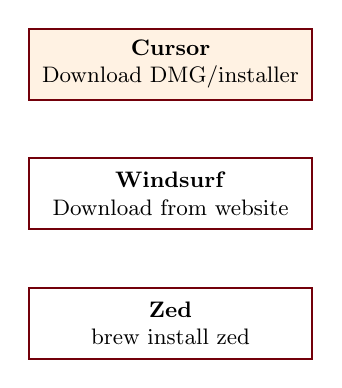
\begin{tikzpicture}[
                    node distance=0.8cm,
                    scale=0.9,
                    transform shape
                ]
                    \node[agentboxfill, minimum width=4cm] (cursor) {
                        \textbf{Cursor}\\
                        \small Download DMG/installer
                    };
                    \node[agentbox, below=of cursor, minimum width=4cm] (windsurf) {
                        \textbf{Windsurf}\\
                        \small Download from website
                    };
                    \node[agentbox, below=of windsurf, minimum width=4cm] (zed) {
                        \textbf{Zed}\\
                        \small brew install zed
                    };
                \end{tikzpicture}
            \end{center}

            \vspace{0.3cm}
            \begin{alertblock}{Time Required}
                10--15 minutes per IDE
            \end{alertblock}
        \end{column}
    \end{columns}

    \note{Installing agentic IDEs is much simpler than terminal agents---you mostly just download and configure your API key.}
\end{frame}

% ----------------------------------------------------------------------------
\begin{frame}[fragile]{Cursor: Installation \& First Launch}
    \begin{columns}[T]
        \begin{column}{0.5\textwidth}
            \begin{block}{System Requirements}
                \begin{itemize}
                    \item macOS 10.12+ OR Linux (Ubuntu 18.04+)
                    \item 2GB RAM (4GB+ recommended)
                    \item 500MB free disk space
                \end{itemize}
            \end{block}

            \begin{block}{Installation --- macOS}
                \begin{lstlisting}[style=bash]
# Option 1: Download from
# https://www.cursor.sh/

# Option 2: Homebrew
brew install cursor

# Verify
/Applications/Cursor.app/Contents/
  MacOS/Cursor --version
                \end{lstlisting}
            \end{block}
        \end{column}
        \begin{column}{0.5\textwidth}
            \begin{block}{Installation --- Linux}
                \begin{lstlisting}[style=bash]
# Ubuntu/Debian
wget https://download.cursor.sh/
  linux -O cursor.deb
sudo dpkg -i cursor.deb

# Or download AppImage
wget https://download.cursor.sh/
  linux/appimage
chmod +x cursor-*.AppImage
./cursor-*.AppImage
                \end{lstlisting}
            \end{block}

            \begin{exampleblock}{First Launch}
                \begin{enumerate}
                    \item Open Cursor.app
                    \item Choose LLM (GPT-4, Claude, etc.)
                    \item Enter API key
                    \item Create/open project
                \end{enumerate}
            \end{exampleblock}
        \end{column}
    \end{columns}

    \note{Cursor installation is straightforward---it's basically a VS Code clone with AI integrated. If you know VS Code, you already know most of Cursor's interface.}
\end{frame}

% ----------------------------------------------------------------------------
\begin{frame}{Cursor: Key Features \& Workflow}
    \begin{columns}[T]
        \begin{column}{0.5\textwidth}
            \begin{block}{Key Features}
                \begin{enumerate}
                    \item \textbf{Cmd+K Code Generation}
                    \begin{itemize}
                        \item Highlight code, press Cmd+K
                        \item Describe changes naturally
                    \end{itemize}
                    \item \textbf{Cmd+L Chat Interface}
                    \begin{itemize}
                        \item Side chat with full context
                        \item Multistep refactoring
                    \end{itemize}
                    \item \textbf{Tab/Autocomplete}
                    \begin{itemize}
                        \item Intelligent completion
                        \item Shows prediction intent
                    \end{itemize}
                    \item \textbf{Agent Mode}
                    \begin{itemize}
                        \item Multi-file changes
                        \item Full refactoring
                    \end{itemize}
                \end{enumerate}
            \end{block}
        \end{column}
        \begin{column}{0.5\textwidth}
            \begin{exampleblock}{Common Workflow}
                \begin{enumerate}
                    \item Open project in Cursor
                    \item Select code to improve
                    \item Press Cmd+K
                    \item Type: ``Refactor to async/await''
                    \item Review changes
                    \item Accept or iterate
                \end{enumerate}
            \end{exampleblock}

            \begin{block}{Pro Tips}
                \begin{itemize}
                    \item Use \texttt{@codebase} for whole project
                    \item Use \texttt{@file name.py} for specific file
                    \item Create Cursor Rules in \texttt{.cursor/rules}
                    \item Custom Instructions for style
                \end{itemize}
            \end{block}
        \end{column}
    \end{columns}

    \note{Cursor is designed for developer comfort. The Cmd+K and Cmd+L shortcuts become second nature quickly.}
\end{frame}

% ----------------------------------------------------------------------------
\begin{frame}[fragile]{Windsurf: Installation \& Features}
    \begin{columns}[T]
        \begin{column}{0.5\textwidth}
            \begin{block}{Installation}
                \begin{lstlisting}[style=bash]
# macOS via Homebrew
brew install windsurf

# Or download from
# https://www.windsurf.dev

# Linux
sudo dpkg -i windsurf.deb

# First launch:
# 1. Select LLM provider
# 2. Enter API key
# 3. Create workspace
                \end{lstlisting}
            \end{block}
        \end{column}
        \begin{column}{0.5\textwidth}
            \begin{block}{Key Differentiators}
                \begin{enumerate}
                    \item \textbf{Cascade Mode}
                    \begin{itemize}
                        \item Multi-file orchestration
                        \item Plans across files
                        \item Shows full diff first
                    \end{itemize}
                    \item \textbf{Flow Feature}
                    \begin{itemize}
                        \item Visualize reasoning
                        \item Step-by-step process
                    \end{itemize}
                    \item \textbf{Workspace Integration}
                    \begin{itemize}
                        \item Full context awareness
                        \item Coordinated changes
                    \end{itemize}
                \end{enumerate}
            \end{block}
        \end{column}
    \end{columns}

    \vspace{0.2cm}
    \begin{exampleblock}{Example Workflow}
        Ask: ``Refactor payments to use dependency injection'' $\rightarrow$ Windsurf analyzes all files $\rightarrow$ Shows Cascade plan $\rightarrow$ You approve $\rightarrow$ All files updated together
    \end{exampleblock}

    \note{Windsurf is newer but impressive. The Cascade feature for multi-file orchestration is particularly powerful.}
\end{frame}

% ----------------------------------------------------------------------------
\begin{frame}[fragile]{Zed: High-Performance Agentic Editor}
    \begin{columns}[T]
        \begin{column}{0.5\textwidth}
            \begin{block}{About Zed}
                \begin{itemize}
                    \item \textbf{Rust-based} (extremely fast)
                    \item Modern architecture
                    \item Emerging agentic features
                    \item Multiplayer editing support
                    \item Lightweight and responsive
                \end{itemize}
            \end{block}

            \begin{block}{Installation}
                \begin{lstlisting}[style=bash]
# macOS via Homebrew
brew install zed

# Or download from
# https://zed.dev

# Linux (requires build)
git clone https://github.com/
  zed-industries/zed
cd zed
cargo install --path crates/zed
                \end{lstlisting}
            \end{block}
        \end{column}
        \begin{column}{0.5\textwidth}
            \begin{block}{Zed Agentic Features}
                \begin{enumerate}
                    \item \textbf{AI Chat Panel}
                    \begin{itemize}
                        \item Right sidebar chat
                        \item Context-aware understanding
                    \end{itemize}
                    \item \textbf{Inline Editing}
                    \begin{itemize}
                        \item Request generation inline
                        \item Immediate visual feedback
                    \end{itemize}
                    \item \textbf{LLM Selection}
                    \begin{itemize}
                        \item Multiple providers
                        \item Easy switching
                    \end{itemize}
                \end{enumerate}
            \end{block}

            \begin{alertblock}{Performance}
                \begin{itemize}
                    \item Starts in $<$1 second
                    \item Instant syntax highlighting
                    \item Snappy navigation
                    \item Minimal memory usage
                \end{itemize}
            \end{alertblock}
        \end{column}
    \end{columns}

    \note{Zed is worth watching. It's the fastest editor in this list and the architecture is superior. However, it's newer and less feature-complete.}
\end{frame}

% ----------------------------------------------------------------------------
\begin{frame}{Agentic IDEs: Side-by-Side Comparison}
    \begin{center}
        \small
        \begin{tabular}{@{}l c c c@{}}
            \toprule
            \textbf{Feature} & \textbf{Cursor} & \textbf{Windsurf} & \textbf{Zed} \\
            \midrule
            Maturity & Mature & Newer & Emerging \\
            Ease of Setup & Very easy & Easy & Medium \\
            VS Code Familiarity & Highest & High & Lower \\
            Multi-file Agentic & Good & \textcolor{Garnet}{\textbf{Excellent}} & Good \\
            Speed & Fast & Medium & \textcolor{Garnet}{\textbf{Very Fast}} \\
            Price & \$20/month & \$30/month & Free tier \\
            Linux Support & Full & Full & Partial \\
            Windows Support & Full & Full & In development \\
            \bottomrule
        \end{tabular}
    \end{center}

    \vspace{0.3cm}
    \begin{columns}[T]
        \begin{column}{0.33\textwidth}
            \begin{block}{Choose Cursor if}
                \begin{itemize}
                    \item Want safest choice
                    \item Know VS Code well
                    \item New to agentic tools
                \end{itemize}
            \end{block}
        \end{column}
        \begin{column}{0.33\textwidth}
            \begin{block}{Choose Windsurf if}
                \begin{itemize}
                    \item Want best agentic
                    \item Complex refactoring
                    \item Budget not concern
                \end{itemize}
            \end{block}
        \end{column}
        \begin{column}{0.33\textwidth}
            \begin{block}{Choose Zed if}
                \begin{itemize}
                    \item Want peak speed
                    \item Like cutting-edge
                    \item Comfortable with new
                \end{itemize}
            \end{block}
        \end{column}
    \end{columns}

    \note{There's no objectively ``best'' choice. Most developers would pick Cursor for stability, but Windsurf and Zed each have compelling reasons.}
\end{frame}

% ============================================================================
% SECTION 5: VS CODE PLUGINS INSTALLATION
% ============================================================================
\section{VS Code Plugins Installation}

% ----------------------------------------------------------------------------
\begin{frame}{VS Code Plugins Overview}
    \begin{columns}[T]
        \begin{column}{0.5\textwidth}
            \begin{block}{Why VS Code Plugins?}
                \begin{itemize}
                    \item Keep your existing editor
                    \item Lower barrier to entry
                    \item Many free/freemium options
                    \item Easy to compare tools
                    \item Familiar environment
                \end{itemize}
            \end{block}

            \begin{block}{Installation Overview}
                \begin{itemize}
                    \item All via Extensions marketplace
                    \item $<$5 minutes each to set up
                    \item Require LLM API keys
                    \item Work alongside normal VS Code
                \end{itemize}
            \end{block}

            \begin{alertblock}{Time Required}
                20--30 minutes total for all four
            \end{alertblock}
        \end{column}
        \begin{column}{0.5\textwidth}
            \begin{center}
                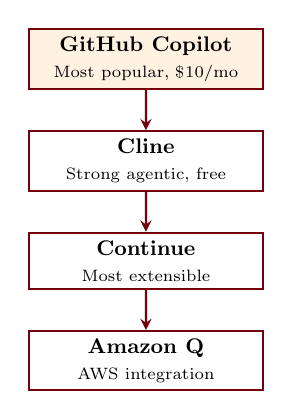
\begin{tikzpicture}[
                    node distance=0.6cm,
                    scale=0.85,
                    transform shape,
                    plugin/.style={agentbox, minimum width=3.5cm, minimum height=0.8cm}
                ]
                    \node[plugin, fill=Sandstorm] (copilot) {
                        \textbf{GitHub Copilot}\\
                        \scriptsize Most popular, \$10/mo
                    };
                    \node[plugin, below=of copilot] (cline) {
                        \textbf{Cline}\\
                        \scriptsize Strong agentic, free
                    };
                    \node[plugin, below=of cline] (continue) {
                        \textbf{Continue}\\
                        \scriptsize Most extensible
                    };
                    \node[plugin, below=of continue] (amazonq) {
                        \textbf{Amazon Q}\\
                        \scriptsize AWS integration
                    };

                    \draw[arrow] (copilot) -- (cline);
                    \draw[arrow] (cline) -- (continue);
                    \draw[arrow] (continue) -- (amazonq);
                \end{tikzpicture}
            \end{center}
        \end{column}
    \end{columns}

    \note{VS Code plugins are the easiest entry point for new users. You don't have to learn a new editor, just add extensions.}
\end{frame}

% ----------------------------------------------------------------------------
\begin{frame}{GitHub Copilot: Installation \& Setup}
    \begin{columns}[T]
        \begin{column}{0.5\textwidth}
            \begin{block}{Prerequisites}
                \begin{itemize}
                    \item VS Code installed
                    \item GitHub account
                    \item Copilot subscription (\$10/mo) OR Free tier
                \end{itemize}
            \end{block}

            \begin{block}{Installation Steps}
                \begin{enumerate}
                    \item Open VS Code
                    \item Click Extensions (Cmd+Shift+X)
                    \item Search ``GitHub Copilot''
                    \item Click Install
                    \item Sign in to GitHub
                    \item Authorize VS Code
                \end{enumerate}
            \end{block}

            \begin{block}{Pricing Tiers}
                \small
                \begin{itemize}
                    \item Free: Chat, limited completions
                    \item Individual: \$10/mo, unlimited
                    \item Business: \$19/user/mo
                \end{itemize}
            \end{block}
        \end{column}
        \begin{column}{0.5\textwidth}
            \begin{exampleblock}{Core Features}
                \begin{enumerate}
                    \item \textbf{Code Completion (Tab)}
                    \begin{itemize}
                        \item Type signature $\rightarrow$ get implementation
                    \end{itemize}
                    \item \textbf{Chat (Cmd+Shift+I)}
                    \begin{itemize}
                        \item Ask questions about code
                        \item Multi-turn conversations
                    \end{itemize}
                    \item \textbf{Inline Comments}
                    \begin{itemize}
                        \item Write what code should do
                        \item Copilot generates it
                    \end{itemize}
                    \item \textbf{Code Explanation}
                    \begin{itemize}
                        \item Select $\rightarrow$ Right-click $\rightarrow$ Explain
                    \end{itemize}
                \end{enumerate}
            \end{exampleblock}

            \begin{block}{Key Keybindings}
                \small
                \texttt{Cmd+Shift+I}: Open chat\\
                \texttt{Tab}: Accept suggestion\\
                \texttt{Escape}: Reject suggestion\\
                \texttt{Alt+]}/\texttt{[}: Next/prev suggestion
            \end{block}
        \end{column}
    \end{columns}

    \note{GitHub Copilot is the market leader because it was first and integrated deeply with GitHub. The free tier is generous for getting started.}
\end{frame}

% ----------------------------------------------------------------------------
\begin{frame}{Cline, Continue, and Amazon Q Setup}
    \begin{columns}[T]
        \begin{column}{0.33\textwidth}
            \begin{block}{Cline}
                \textbf{Installation:}
                \begin{enumerate}
                    \item Extensions $\rightarrow$ ``Cline''
                    \item Install
                    \item Settings $\rightarrow$ API Key
                    \item Click Cline icon
                \end{enumerate}

                \vspace{0.2cm}
                \textbf{Strengths:}
                \begin{itemize}
                    \item Multi-file editing
                    \item Strong reasoning
                    \item Many LLM providers
                    \item Free/freemium
                \end{itemize}
            \end{block}
        \end{column}
        \begin{column}{0.33\textwidth}
            \begin{block}{Continue}
                \textbf{Installation:}
                \begin{enumerate}
                    \item Extensions $\rightarrow$ ``Continue''
                    \item Install
                    \item Select LLM provider
                    \item Enter API key
                \end{enumerate}

                \vspace{0.2cm}
                \textbf{Strengths:}
                \begin{itemize}
                    \item Most customizable
                    \item Open-source core
                    \item Great documentation
                    \item Works with Ollama
                \end{itemize}
            \end{block}
        \end{column}
        \begin{column}{0.33\textwidth}
            \begin{block}{Amazon Q}
                \textbf{Installation:}
                \begin{enumerate}
                    \item Extensions $\rightarrow$ ``Amazon Q''
                    \item Install
                    \item Sign in with AWS
                    \item Authorize
                \end{enumerate}

                \vspace{0.2cm}
                \textbf{Strengths:}
                \begin{itemize}
                    \item AWS integration
                    \item Free for individuals
                    \item Enterprise support
                    \item AWS documentation
                \end{itemize}
            \end{block}
        \end{column}
    \end{columns}

    \vspace{0.2cm}
    \begin{exampleblock}{Quick Start Recommendation}
        1. Install \textbf{GitHub Copilot} first (familiar) \quad
        2. Try \textbf{Cline} for more agentic \quad
        3. Experiment with \textbf{Continue} for customization
    \end{exampleblock}

    \note{Different plugins excel at different tasks. Many developers install all four and use them contextually.}
\end{frame}

% ----------------------------------------------------------------------------
\begin{frame}{Complete Setup Workflow}
    \begin{columns}[T]
        \begin{column}{0.5\textwidth}
            \begin{block}{Recommended Order (60--90 min)}
                \textbf{Phase 1: Terminal Agents (30--40 min)}
                \begin{itemize}
                    \item Claude Code (10 min)
                    \item Aider (5 min)
                    \item Gemini CLI or Codex CLI (10 min)
                    \item Test each (5--10 min)
                \end{itemize}

                \textbf{Phase 2: One Agentic IDE (10--15 min)}
                \begin{itemize}
                    \item Download \& install (5 min)
                    \item Configure API keys (3 min)
                    \item Test features (5 min)
                \end{itemize}

                \textbf{Phase 3: VS Code Plugins (20--30 min)}
                \begin{itemize}
                    \item GitHub Copilot (5 min)
                    \item Cline (5 min)
                    \item Continue (5 min)
                    \item Test each (5--10 min)
                \end{itemize}
            \end{block}
        \end{column}
        \begin{column}{0.5\textwidth}
            \begin{exampleblock}{Verification Checklist}
                \textbf{Terminal Agents:}
                \begin{itemize}
                    \item[$\square$] Claude Code accepts prompts
                    \item[$\square$] Aider modifies code
                    \item[$\square$] Gemini/Codex responds
                    \item[$\square$] All API keys configured
                \end{itemize}

                \textbf{IDE:}
                \begin{itemize}
                    \item[$\square$] Launches without errors
                    \item[$\square$] Chat interface responds
                    \item[$\square$] Code generation works
                \end{itemize}

                \textbf{VS Code Plugins:}
                \begin{itemize}
                    \item[$\square$] All plugins installed
                    \item[$\square$] Each shows connected status
                    \item[$\square$] Test prompts work
                \end{itemize}
            \end{exampleblock}
        \end{column}
    \end{columns}

    \note{This is ambitious---8+ different tools by the end. Most developers settle on 3--4 favorites, but having tried them all gives you perspective.}
\end{frame}

% ============================================================================
% SECTION 6: SUMMARY & NEXT STEPS
% ============================================================================
\section{Summary \& Next Steps}

% ----------------------------------------------------------------------------
\begin{frame}{Part 1 Summary: What You've Learned}
    \begin{columns}[T]
        \begin{column}{0.5\textwidth}
            \begin{block}{1. Agentic Tools Fundamentals}
                \begin{itemize}
                    \item What agentic tools are
                    \item How they differ from traditional AI
                    \item The agent loop: observe, plan, execute, refine
                \end{itemize}
            \end{block}

            \begin{block}{2. The Three Categories}
                \begin{itemize}
                    \item Terminal-based agents (most powerful)
                    \item Agentic IDEs (optimized editors)
                    \item VS Code plugins (integrated approach)
                \end{itemize}
            \end{block}

            \begin{block}{3. Specific Tools Covered}
                \begin{itemize}
                    \item 8+ terminal agents
                    \item 3 agentic IDEs
                    \item 4 VS Code plugins
                \end{itemize}
            \end{block}
        \end{column}
        \begin{column}{0.5\textwidth}
            \begin{exampleblock}{Tools You've Installed}
                \textbf{Terminal Agents:}
                \begin{itemize}
                    \item[$\square$] Claude Code
                    \item[$\square$] Aider
                    \item[$\square$] Gemini CLI
                    \item[$\square$] Codex CLI
                \end{itemize}

                \textbf{IDEs:}
                \begin{itemize}
                    \item[$\square$] Cursor (recommended)
                \end{itemize}

                \textbf{VS Code Plugins:}
                \begin{itemize}
                    \item[$\square$] GitHub Copilot
                    \item[$\square$] Cline
                    \item[$\square$] Continue
                \end{itemize}
            \end{exampleblock}
        \end{column}
    \end{columns}

    \note{You've just installed a comprehensive toolkit. Different tools will click with different people---that's normal.}
\end{frame}

% ----------------------------------------------------------------------------
\begin{frame}{Next Steps \& Resources}
    \begin{columns}[T]
        \begin{column}{0.5\textwidth}
            \begin{block}{Part 2 Preview: Workflows \& Best Practices}
                Coming up:
                \begin{enumerate}
                    \item Effective prompting techniques
                    \item Multi-step problem solving
                    \item Git and CI/CD integration
                    \item When to use which tool
                    \item Advanced patterns
                \end{enumerate}
            \end{block}

            \begin{exampleblock}{Your Challenge for Part 2}
                \begin{enumerate}
                    \item Pick a small project from GitHub
                    \item Ask each tool: ``Identify potential bugs''
                    \item Compare responses
                    \item Notice which was most helpful
                    \item Understand why
                \end{enumerate}
            \end{exampleblock}
        \end{column}
        \begin{column}{0.5\textwidth}
            \begin{block}{Official Documentation}
                \small
                \begin{itemize}
                    \item Claude Code: \url{docs.anthropic.com}
                    \item Aider: \url{aider.chat/docs}
                    \item Cursor: \url{docs.cursor.sh}
                    \item Windsurf: \url{windsurf.dev/docs}
                \end{itemize}
            \end{block}

            \begin{block}{Community Resources}
                \small
                \begin{itemize}
                    \item Anthropic Discord
                    \item Aider GitHub Discussions
                    \item Cursor Discord
                    \item Continue Slack community
                \end{itemize}
            \end{block}
        \end{column}
    \end{columns}

    \vspace{0.2cm}
    \begin{alertblock}{Key Takeaway}
        The real learning begins in Part 2. These tools are installed---now learn to use them \textbf{effectively}.
    \end{alertblock}

    \note{In Part 2, we'll focus on how to use these tools effectively, not just how to install them.}
\end{frame}

% ----------------------------------------------------------------------------
\begin{frame}[plain]
    \begin{center}
        \vspace{2cm}
        {\Huge\textcolor{Garnet}{\textbf{End of Part 1}}}

        \vspace{1cm}
        {\Large Introduction \& Installation}

        \vspace{1cm}
        {\large Questions?}

        \vspace{2cm}
        {\small
            \textcolor{Atlantic}{Part 2: Workflows \& Best Practices} --- Coming Next
        }
    \end{center}
\end{frame}

% ============================================================================
% DOCUMENT END
% ============================================================================
\end{document}
